\section{Perceptrón}

El perceptrón fue la primera red neuronal artificial (o ANS, Artificial Neural Systems) descrita algoritmicamente. En las decadas de los 60's y 70's, los popularizo el psicólogo Franck Rosenblatt, en su libro llamado Principios de neurodinámica, donde presentó varios modelos de perceptrones, en el Laboratorio Aeronáutico de Cornell en Estados Unidos, originalmente estaba diseñado para ser una máquina, en vez de un algoritmo. Estaba diseñado especificamete para el reconocimiento de imagenes donde, cada peso era un cable físico por pixel de entrada, este erá una matriz de 200 x 200, conectados aleatoriamente a las "neuronas", las actualizaciones de los pesos se realizarón mediante motores eléctricos. 

El perceptrón es en sí, es la representación de un sola neurona, este se ocupa para la clasificación de patrones en un conjunto de datos multivariados, con ese se obtienen fronteras lineales en el plano, mediante un algoritmo de aprendizaje que veremos más adelante.

Recordando, una neurona es un celula elemental que a partir de un vector de entrada procedente del exterior o de otras neuronas (estimulo), proporciona una única respuesta (si activo el potencial de acción o no), ver figura \ref{fig:unaNeurona}. Los elementos que actuan en una neurona los podemos listar como:
\begin{itemize}
 \item \textbf{Entradas:} $x_{j}(t)$. Las variables de entrada y salida pueden ser binarias (digitales) o continuas (analógicas) dependiendo del modelo de aplicación.
 \item \textbf{Pesos sinápticos:} $w_{ij}$. Representan la intensidad de interacción entre cada neurona presináptica j y la neurona postsináptica i.
 \item \textbf{Regla de propagación:} $h_{i}(t) = \sigma(w_{ij}, x_{j}(t))$. Proporciona el valor del potencial postsináptico, de la neurona i en función de sus pesos y entradas. 
    \begin{itemize}
     \item $h_{i}(t) = \sum_{i=0}^{n} w_{ij} x_{i} $, Es una suma ponderada de las entradas con los pesos sinápticos.
      Así, si la entrada es positiva, dependiendo de los pesos podemos saber si fue una sinapsis excitadora (pesos positivos) o inhibidora (pesos negativos).
    \end{itemize}

 \item \textbf{Función de activación o de transferencia:} $a_{i}(t)$ Proporciona el estado de activación actual, de la neurona $i$ en función de su estado anterior, $a_{i}(t-1)$ y de su potencial postsináptico actual. 
    \begin{itemize}
     \item $a_{i}(t) = f_{i}(a_{i}(t-1),h_{i}(t))$, es la que usalmente se usa.
     \item $a_{i}(t) = f_{i}(h_{i}(t))$, en algunos modelos solo se concidera que el estado actual no dependende del tiempo anterior.

     \end{itemize}

 \item \textbf{Función de salida: } $F_{i}(a_{i}(t))$ Da la salida actual, $y_{i}(t)$, de la neurona i en función de su estado de activación actual. El estado de activación de la neurona se considera como la propia salida. 
    \begin{itemize}
     \item $y_{i}(t) = F_{i}(a_{i}(t))$
     \item $y_{i}(t) = F_{i}(f_{i}(a_{i}(t-1),\sigma(w_{ij},x_{j}(t))))$
    \end{itemize}

\end{itemize}


\begin{figure}[h]
 \centering
 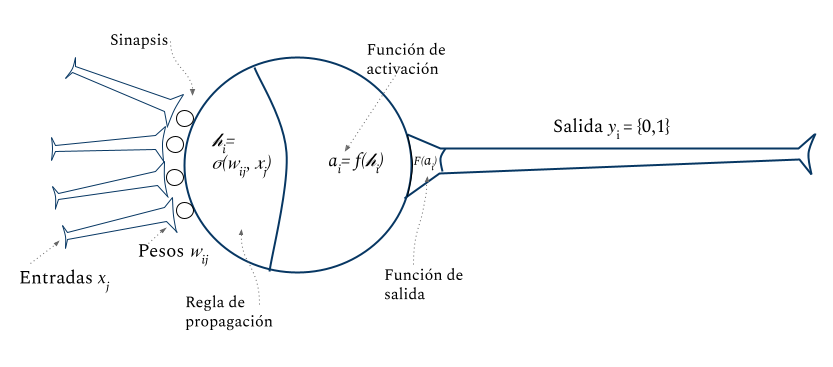
\includegraphics[scale=0.5]{../Figuras/Percp.png}
 \caption{Neurona vista como un modelo artificial (perceptrón).}
 \label{fig:unaNeurona}
\end{figure}


Un perceptrón toma un vector de entradas de numeros reales, calcula una combinación lineal de estas entradas, luego emite un 1 si el resultado es mayor que algún umbral y -1 de lo contrario. 
Es decir, dadas las entradas $x_{1}... x_{n}$, la salida $o(x_{1}. ..., x_{n})$ calculada por el perceptrón es 1 si $w_{0} + w_{1}x_{1} + w_{2}x_{2} + ... + w_{n}x_{2} > 0 $ y -1 de lo contrario, donde cada $w$ es una constante $\mathbb{R}$, un peso, que determina la contribución de la entrada $x$ a la salida del perceptrón.  La constante $w_{0}$ es un \emph{umbral} (bias) que la suma de las entradas con los pesos debe superar para que el perceptrón emita un 1. En otras palabras es un peso que va a actuar junto con una entrada de valor $1$, que vamos a poder ajustar para que nuestrá función de activación, se mueva de derecha a izquierda en el plano para ayudarnos a ajustar nuestros resultados, provocando un gran impacto en el aprendizaje. Esto se muestra en la siguientes graficas \ref{fig:bias}. Más adelante hablaremos de su regla de entrenamiento (Training rule).

\begin{figure}[h]
    %\centering
    \subfloat[Función sigmoide.]{
            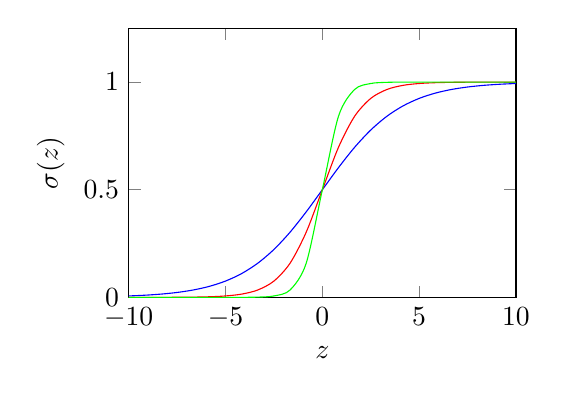
\begin{tikzpicture}
            \begin{axis}[width=6.5cm,height=5cm,ylabel=$\sigma(z)$,xlabel=$z$,ymin=0,ymax=1.25,xmin=-10,xmax=10]
                \addplot[domain=-10:10,blue,smooth] {1/(1+exp(-(x*.5)))};
                \addplot[domain=-10:10,red,smooth] {1/(1+exp(-(x* 1)))};
                \addplot[domain=-10:10,green,smooth] {1/(1+exp(-(x* 2)))};
                %\addlegendentry{$y = \dfrac{1}{1+e^{-x}}$}
            \end{axis}
        \end{tikzpicture}
    }
    \subfloat[Función sigmoide con bias.]{
            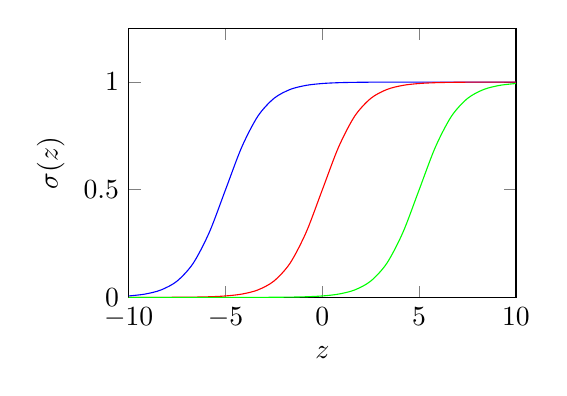
\begin{tikzpicture}
            \begin{axis}[width=6.5cm,height=5cm,ylabel=$\sigma(z)$,xlabel=$z$,ymin=0,ymax=1.25,xmin=-10,xmax=10]
                \addplot[domain=-10:10, blue,smooth] {1/(1+exp(-(x*1 + 5)))};
                \addplot[domain=-10:10, red,smooth] {1/(1+exp(-(x* 1)))};
                \addplot[domain=-10:10, green,smooth] {1/(1+exp(-(x* 1 - 5)))};

                %\addlegendentry{$w = -5$}
            \end{axis}
        \end{tikzpicture}
    \label{fig:bias}
    }
    \caption[Impacto del bias]{
     Comportamiento de la función de activación (sigmoide) de un perceptrón con una sola entrada, \emph{(b)} el perceptrón sin el uso de bias, \emph{(b)} con el uso del bias, donde apesar de estár representandos con la misma entrada , el uso del bias afecta en los resultados de salida. Así si quisieramos que este perceptrón nos diera $y = 0$ con una entrada $x= 2$ sin el uso, ni ajuste del bias sería imposible, pues en (a) apesar que la gráfica azul está la entrada está ajustada con el peso $w=0.5$, la roja con el $w=1$, y la verde con el $w=2$  solo lo gramos alargarla un poco, haciendo que entradas que antes eran correctas ahora caigan $0$ también. Entonces lo que necesitamos es más bien "mover" la gráfica, esto lo logramos con la gráfica \emph{(b)} donde la entrada (única) está sumada con un bias (umbral) $x_{0}= 1$, ajustado en azul con peso $w_{0}= 5$, en rojo con $w_{0}= 0$, en verde con $w_{0}= -5$ y el peso $w_{1}=1$. Donde con $w_{0}= -5$ logramos nuestro objetivo de tener una salida $y=0$ con $x=2$. El bias nos permite mover la función fuera del origen.
     \label{fig:sigmoideBias}
     }
\end{figure}


El hecho de que un perceptrón aprenda implica elegir valores para los pesos denotados también por $\theta$.  Ahora, el espacio $H$ de las hipótesis candidatas consideradas en el aprendizaje del perceptrón, es el conjunto de todos los posibles vectores de pesos.  \[H = {\vec{w} |  \vec{w} \in \mathbb{R}^{n+1}}\].

\begin{figure}[h]
 \centering
 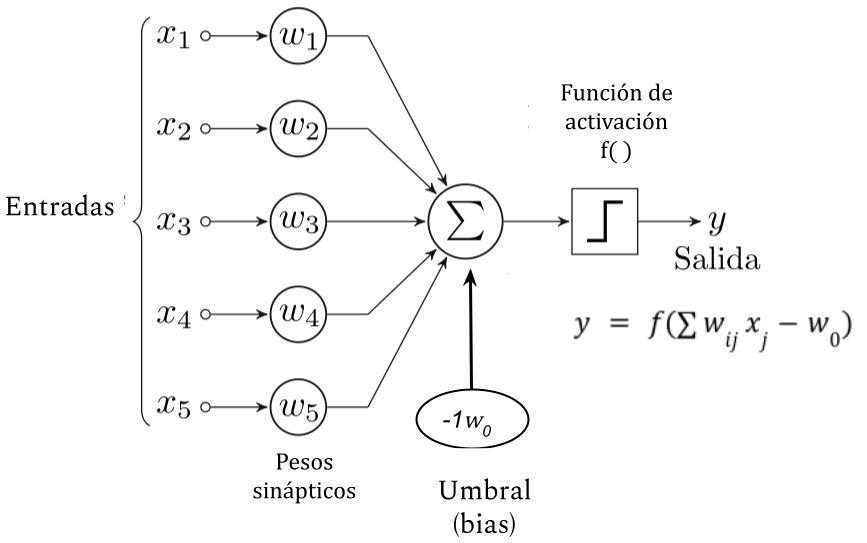
\includegraphics[scale=0.5]{../Figuras/Perceptron.png}
 \caption{Modelo estandar de un perceptrón.}
 \label{fig:unaNeurona2}
\end{figure}

Si bien en el momento que se publicó los logros con el modelo del percetrón las espectativas eran bastante altas, a medida de los años los cientificos Marvin Minsky and Seymour Papert desestiman en gran medida los alcances que realmente se puede tener con el perceptrón, al mostrar \footnote{ En 1969 publican Marvin Minsky y Seymour Papert que perceptrones de una sola capa (simples) solo son capaces de aprender a distinguir patrones linealmente separables, en el libro "Perceptrons".
} que no puede predecir operaciones lógicas que no sean linealmente separables, tal es el caso de la función XOR, que no es separable linealmente, siendo imposible que pueda aprender está función. Esto y el gran costo que representaba procesar todos los elementos que implicaba el entrenamiento, causa que por un buen tiempo se desetime el uso del perceptrón. Es hasta después de unas decadas que vuelve a tener relevancia con la propuesta de un perceptrón multicapa usando retropagación (Feedforward), siendo estos capaces de resolver la función XOR


